\documentclass[11pt,a4paper]{article}

\usepackage{iftex}
\ifPDFTeX
  \usepackage[utf8]{inputenc}
  \usepackage[T1]{fontenc}
  \usepackage{newtxtext}
  \usepackage{newtxmath}
\else
  \usepackage{fontspec}
  \setmainfont{Times New Roman}
\fi
\usepackage[a4paper,top=2.4cm,bottom=2.4cm,left=2.35cm,right=2.35cm,headheight=22pt]{geometry}
\ifPDFTeX
  \usepackage[protrusion=true,expansion=true]{microtype}
\else
  \usepackage[protrusion=true]{microtype}
\fi
\usepackage{graphicx}
\usepackage{array}
\usepackage{booktabs}
\usepackage{tabularx}
\usepackage{longtable}
\usepackage{enumitem}
\usepackage{hyperref}
\usepackage[table]{xcolor}
\usepackage{titlesec}
\usepackage{fancyhdr}
\usepackage{parskip}
\usepackage{tikz}
\usepackage{tcolorbox}
\tcbuselibrary{skins}

% Monochrome proposal palette
\definecolor{spotgreen}{HTML}{000000}
\definecolor{spotlight}{HTML}{000000}
\definecolor{spotbg}{HTML}{F7F7F7}
\definecolor{spotdark}{HTML}{000000}
\definecolor{spotgray}{HTML}{000000}
\definecolor{rulegray}{HTML}{D7DDD8}

\linespread{1.035}
\setlength{\parskip}{0.55em}
\setlength{\parindent}{0pt}
\emergencystretch=2em
\setlength{\tabcolsep}{6pt}
\renewcommand{\arraystretch}{1.18}
\newcolumntype{Y}{>{\raggedright\arraybackslash}X}
\setlist[itemize]{leftmargin=1.4em,itemsep=0.18em,topsep=0.25em}
\setlist[enumerate]{leftmargin=1.6em,itemsep=0.18em,topsep=0.25em}
\setlength{\arrayrulewidth}{0.4pt}
\newcommand{\proposalTableStart}{\arrayrulecolor{black}}
\newcommand{\proposalTableHeader}{}
\newcommand{\proposalTableEnd}{\arrayrulecolor{black}}

% Hyperlink styling
\hypersetup{
  colorlinks=true,
  linkcolor=spotgreen,
  urlcolor=spotgreen,
  citecolor=spotgreen,
  pdftitle={Spotree -- Proposal for TreeQuest Challenge},
  pdfauthor={Spotree Team}
}

% Section styling
\setcounter{secnumdepth}{3}
\setcounter{tocdepth}{2}
\titleformat{\section}
  {\normalfont\fontsize{18}{22}\selectfont\bfseries}
  {\thesection.}{0.65em}{}
\titleformat{\subsection}
  {\normalfont\fontsize{14}{17}\selectfont\bfseries}
  {\thesubsection}{0.75em}{}
\titleformat{\subsubsection}
  {\normalfont\fontsize{12}{15}\selectfont\bfseries\itshape}
  {\thesubsubsection}{0.65em}{}
\titlespacing*{\section}{0pt}{0.6em}{1.0em}
\titlespacing*{\subsection}{0pt}{1.25em}{0.65em}
\titlespacing*{\subsubsection}{0pt}{1.0em}{0.45em}

% Header/footer
\pagestyle{fancy}
\fancyhf{}
\fancyhead[L]{\footnotesize\color{spotgray}\MakeUppercase{Spotree Proposal}}
\fancyhead[R]{\footnotesize\color{spotgray}TreeQuest Challenge \enspace | \enspace \thepage}
\fancyfoot[C]{\footnotesize\color{spotgray}Munich Innovation Challenge 2026}
\renewcommand{\headrulewidth}{0.3pt}
\renewcommand{\footrulewidth}{0pt}
\renewcommand{\headrule}{\hbox to\headwidth{\color{rulegray}\leaders\hrule height \headrulewidth\hfill}}

\begin{document}
\hypersetup{pageanchor=false}

% ── Title Page ──
\begin{titlepage}
\thispagestyle{empty}
\centering
\vspace*{2.4cm}

{\small\bfseries\color{spotgreen}\MakeUppercase{Proposal for the TreeQuest Challenge}\par}
\vspace{0.6cm}
{\fontsize{34}{39}\selectfont\bfseries\color{spotdark} Spotree\par}
\vspace{0.35cm}
{\Large\color{spotgray} Student-led tree mapping for Munich's geospatial data infrastructure\par}

\vspace{1.4cm}

\textcolor{spotgreen}{\rule{0.68\textwidth}{0.9pt}}

\vspace{1.4cm}

\begin{tabular}{>{\bfseries\color{spotdark}}r@{\hspace{1.2em}}l}
Prepared for & Munich Innovation Challenge 2026 \\
Theme & Students on an Urban Data Mission \\
Submitted by & Spotree Team \\
Date & May 2026 \\
Source Code & \href{https://github.com/jayepraveen999/spotree/tree/main}{github.com/jayepraveen999/spotree} \\
\end{tabular}

\vfill

{\small\color{spotgray}
An educational, standards-ready mobile application for crowdsourced urban tree data collection.}
\end{titlepage}

% ── Table of Contents ──
\pagenumbering{roman}
\tableofcontents
\newpage
\pagenumbering{arabic}
\hypersetup{pageanchor=true}

% ══════════════════════════════════════════════════════════════
\section{Team}

\vspace{0.3cm}

\newlength{\cardheight}
\setlength{\cardheight}{16.5cm}
\noindent
\begin{minipage}[t]{0.48\textwidth}
\begin{tcolorbox}[
  enhanced, colback=white, colframe=rulegray, arc=2pt, boxrule=0.6pt,
  top=10pt, bottom=10pt, left=11pt, right=11pt, height=\cardheight,
]
\centering
\begin{tikzpicture}
  \clip (0,0) circle (1.6cm);
  \node at (0,0.4) {
\includegraphics[width=3.2cm]{jayendra.jpeg}};
\end{tikzpicture}

\vspace{6pt}
{\large\bfseries\color{spotdark} Jayendra Praveen Kumar}

\vspace{2pt}
{\scriptsize\color{spotgreen}\textbf{LEAD DEVELOPER\enspace$\cdot$\enspace APPLIED RESEARCH}}

\vspace{4pt}
{\small\itshape Applied Research Engineer, OroraTech (Munich) $\cdot$ M.Sc.\ ESPACE, TU Munich}

\vspace{6pt}
\textcolor{rulegray}{\rule{\linewidth}{0.4pt}}
\vspace{4pt}

\raggedright
{\scriptsize\bfseries\color{spotdark} EXPERTISE}

\vspace{4pt}
{\small Applied research in Earth observation, MLOps and real-time inference pipelines for satellite-based wildfire detection. \textbf{Tree species classification using satellite imagery} (university project at TUM under Prof.\ Xiaoxiang Zhu). Published at \textbf{ESA Living Planet Symposium 2025} and \textbf{ECAI 2020}.}

\vspace{6pt}
{\small\textbf{Focus areas:} Deep Learning, PostGIS, Geospatial Data Engineering, Python, PyTorch, Grafana, Docker, Full-Stack App Development.}

\vfill
\textcolor{rulegray}{\rule{\linewidth}{0.4pt}}
\vspace{2pt}
{\scriptsize\color{spotgray} \href{https://linkedin.com/in/jayendrapraveen}{linkedin.com/in/jayendrapraveen}\\
\href{https://github.com/jayepraveen999}{github.com/jayepraveen999}}
\end{tcolorbox}
\end{minipage}%
\hfill
\begin{minipage}[t]{0.48\textwidth}
\begin{tcolorbox}[
  enhanced, colback=white, colframe=rulegray, arc=2pt, boxrule=0.6pt,
  top=10pt, bottom=10pt, left=11pt, right=11pt, height=\cardheight,
]
\centering
\begin{tikzpicture}
  \clip (0,0) circle (1.6cm);
  \node at (0,0) {
\includegraphics[width=3.2cm]{hari.jpeg}};
\end{tikzpicture}

\vspace{6pt}
{\large\bfseries\color{spotdark} Hari Krishna Gadi}

\vspace{2pt}
{\scriptsize\color{spotgreen}\textbf{INITIATIVE\enspace$\cdot$\enspace ARCHITECTURE\enspace$\cdot$\enspace IMPLEMENTATION}}

\vspace{4pt}
{\small\itshape PhD Researcher, Huawei Technologies $\cdot$ M.Sc.\ Geodesy \& Geoinformation, TU Munich}

\vspace{6pt}
\textcolor{rulegray}{\rule{\linewidth}{0.4pt}}
\vspace{4pt}

\raggedright
{\scriptsize\bfseries\color{spotdark} EXPERTISE}

\vspace{4pt}
{\small\textbf{Publications:} First author at \textbf{ICLR 2026} (HierLoc, image-based geolocation in hyperbolic space) and \textbf{SIGSPATIAL '24} (road-network matching with embeddings). Co-author at \textbf{EMNLP 2025} (Turnback, geospatial cognition of current LLMs).}

\vspace{6pt}
{\small\textbf{Focus areas:} Agentic AI, Multimodal LLMs, Proactive Agents, Deep Learning for Spatial Data, GPU Cluster Administration, Rust PostgreSQL Extensions.}

\vfill
\textcolor{rulegray}{\rule{\linewidth}{0.4pt}}
\vspace{2pt}
{\scriptsize\color{spotgray} \href{https://linkedin.com/in/hari-krishna-gadi}{linkedin.com/in/hari-krishna-gadi}\\
\href{https://harikrishnagadi.github.io}{harikrishnagadi.github.io}}
\end{tcolorbox}
\end{minipage}

\vspace{0.6cm}

\noindent
We are a two-person Munich team with complementary strengths. On one side, ML research and full-stack systems engineering. On the other, applied Earth observation and MLOps experience with real-time satellite pipelines. Both of us have been working and researching in Munich for years. We understand the local context, the TU Munich research ecosystem, and the requirements for GDPR-compliant geospatial infrastructure. The Spotree team brings over a decade of combined expertise in geospatial science, earth observation, machine learning, and spatial data infrastructure. Once selected for the co-creation phase, we are eager to refine the concept together with students and teachers, iterate on the prototype based on real-world feedback, and release a production-ready app to the students of Munich.

% ══════════════════════════════════════════════════════════════
\clearpage
\section{Executive Summary}

\textbf{Spotree} (Spotify + Tree) is a mobile application that transforms urban tree mapping into an engaging, social experience for Munich's students. Instead of treating data collection as a chore, Spotree lets students ``spot'' trees, capture rich geospatial data, and \textbf{drop their favorite Spotify song at each tree location} --- creating a musical map of Munich's urban forest.

The name says it all: \textbf{Spo}(tify) + \textbf{tree}. Every tree becomes a point on the map with a soundtrack. When students explore trees mapped by their peers, they can tap to play the linked song. This social, music-driven mechanic gives students a personal reason to keep mapping --- they want to see their song on the map, share it with friends, and discover what others have linked. It turns a civic data project into something students genuinely want to participate in.

Behind the fun interface, Spotree builds a \textbf{production-grade geospatial database} using PostGIS with OGC-compliant spatial data types, ready for direct integration into Munich's existing geodata infrastructure.

% ══════════════════════════════════════════════════════════════
\clearpage
\section{Challenge Response}

The challenge asks: \textit{How can we involve students in Munich in the creation and updating of the city's geospatial data in an active and educational way, while strengthening their connection to their neighbourhood?}

Spotree addresses every dimension of this question:

\begin{center}
\small
\proposalTableStart
\begin{tabularx}{\textwidth}{|>{\bfseries\raggedright\arraybackslash}p{0.29\textwidth}|Y|}
\hline
\proposalTableHeader
\textbf{Challenge Requirement} & \textbf{Spotree Solution} \\
\hline
Crowdsourced data collection & Students capture tree photos, GPS-tagged locations, species identification, health assessment, height estimation, and trunk diameter --- all through a guided mobile form \\
\hline
Educational value & The Spotree Guide teaches 12 native Munich tree species with photos, growth characteristics, habitat info, and links to botanical references (Easyscape). Students learn to identify species before they map \\
\hline
Active participation & The Spotify integration creates intrinsic motivation. Students map trees to drop songs. School-level analytics enable teachers to integrate mapping into lessons \\
\hline
AI integration & Current prototype uses AI (LLaVA vision model) to validate uploaded photos contain trees. Co-creation phase adds AI-powered species classification \\
\hline
Neighbourhood connection & Students explore trees in their area, discover songs left by peers, and build a personal profile. The map becomes a living, musical portrait of their neighbourhood \\
\hline
Rewarding / ranking & Profile tracks trees spotted, species found, and songs shared. Co-creation phase adds leaderboards and area ownership mechanics \\
\hline
OGC-compliant data & All spatial data stored as PostGIS \texttt{geography(Point, 4326)} --- standard WGS84. Export to GeoJSON, Shapefile, GeoParquet supported natively \\
\hline
Verification \& updates & AI rejects non-tree photos. Confidence sliders on every field signal data quality. Multiple students can map the same tree, enabling cross-verification \\
\hline
\end{tabularx}
\proposalTableEnd
\end{center}

% ══════════════════════════════════════════════════════════════
\clearpage
\section{App Description}

Spotree is built as a native iOS app (React Native + Expo) with 5 main tabs:

\subsection{Map}
The central view showing all spotted trees across Munich on an interactive map. Each tree marker indicates its location; markers with a music badge have a linked Spotify song. Tapping a marker opens a detail card showing species, health, height, who mapped it, and a play button for the linked song.

\begin{center}\fbox{\parbox{0.8\linewidth}{\centering\vspace{1.5cm}\textit{[Screenshot: Map View]}\vspace{1.5cm}}}\end{center}

\subsection{Capture (Spot a Tree)}
The guided data collection form. Students can:
\begin{itemize}
  \item \textbf{Take a photo} (camera) or \textbf{pick from gallery} (with EXIF GPS extraction)
  \item AI validates the photo contains a tree before proceeding
  \item Select \textbf{tree species} from 58 Munich natives (or ``Not Sure'' if uncertain)
  \item Rate \textbf{health status} (Healthy / Fair / Poor / Dead)
  \item Estimate \textbf{tree height} and \textbf{trunk diameter}
  \item Set \textbf{confidence levels} (0--100\%) for each observation via sliders
  \item Add \textbf{free-text notes} about the tree or its surroundings
  \item \textbf{Link a Spotify song} --- paste a URL and name the track
\end{itemize}

After submission, the tree appears on the map for all users.

\begin{center}\fbox{\parbox{0.8\linewidth}{\centering\vspace{1.5cm}\textit{[Screenshot: Capture Form]}\vspace{1.5cm}}}\end{center}

\subsection{Explore}
A social feed of recently spotted trees, sorted by time. Each card shows the tree photo, species, health, height, confidence bar, mapper's name, and linked song with a play button. A \textbf{``View on Map''} button zooms directly to any tree's location on the map.

\begin{center}\fbox{\parbox{0.8\linewidth}{\centering\vspace{1.5cm}\textit{[Screenshot: Explore Feed]}\vspace{1.5cm}}}\end{center}

\subsection{Spotree Guide}
An educational reference for Munich's native tree species:
\begin{itemize}
  \item \textbf{12 species} with common and scientific names
  \item \textbf{Swipeable image galleries} with multiple photos per species
  \item \textbf{Fullscreen image viewer} for detailed examination
  \item Plant description chips: height, width, growth rate, flower color, blooming season, leaf retention
  \item Growth requirements: sun exposure, drainage needs
  \item Natural habitat description and common uses
  \item \textbf{External link to Easyscape} for deeper botanical learning
\end{itemize}

Data sourced from Easyscape, a botanical reference platform with verified species information.

\begin{center}\fbox{\parbox{0.8\linewidth}{\centering\vspace{1.5cm}\textit{[Screenshot: Spotree Guide]}\vspace{1.5cm}}}\end{center}

\subsection{Profile}
Personal dashboard showing:
\begin{itemize}
  \item \textbf{Trees Spotted} --- total count
  \item \textbf{Songs Shared} --- trees with linked songs
  \item \textbf{Species Found} --- unique species identified
  \item List of all personally mapped trees with dates and health status
  \item School affiliation (set once during registration)
\end{itemize}

\begin{center}\fbox{\parbox{0.8\linewidth}{\centering\vspace{1.5cm}\textit{[Screenshot: Profile]}\vspace{1.5cm}}}\end{center}

\subsection{Admin Analytics Dashboard}

The admin dashboard is a web application designed for teachers, city administrators, and GeodataService staff to monitor the project at a glance. It connects to the same database as the mobile app and displays live data.

\textbf{Layout:} Stats panel on the left, full interactive map on the right --- no scrolling needed. Grafana-inspired dark theme for comfortable monitoring.

\textbf{Panels:}
\begin{itemize}
  \item \textbf{Stats Strip} --- Total trees, registered users, unique species found, songs linked (with weekly deltas)
  \item \textbf{Species Breakdown} --- Ranked list of all identified species with distribution bars
  \item \textbf{School Analytics} --- Trees per school, showing which schools are most actively participating
  \item \textbf{Health Overview} --- Distribution of tree health statuses across all observations
  \item \textbf{Activity Feed} --- Real-time stream of the latest tree submissions with timestamps, species, and linked songs
  \item \textbf{Interactive Map} --- All trees plotted on a dark-themed map with popups showing full details
\end{itemize}

\textbf{School-level analytics} are particularly valuable: they show which schools and neighborhoods are actively engaged, help identify coverage gaps, and enable targeted outreach to underrepresented areas.

\begin{center}\fbox{\parbox{0.8\linewidth}{\centering\vspace{1.5cm}\textit{[Screenshot: Admin Dashboard]}\vspace{1.5cm}}}\end{center}

% ══════════════════════════════════════════════════════════════
\clearpage
\section{Data Collection \& Value for GeodataService Munich}

Every tree entry in Spotree captures a comprehensive dataset designed to be directly useful for Munich's GeodataService:

\begin{center}
\small
\proposalTableStart
\begin{tabularx}{\textwidth}{|>{\raggedright\arraybackslash}p{0.23\textwidth}|>{\raggedright\arraybackslash}p{0.24\textwidth}|Y|}
\hline
\proposalTableHeader
\textbf{Field} & \textbf{Type} & \textbf{Purpose} \\
\hline
GPS Location & PostGIS Point (4326) & Precise tree position from camera GPS or EXIF metadata \\
\hline
Photo & Image URL & Visual verification of tree existence and condition \\
\hline
Species & Text (58 natives) & Tree species identification \\
\hline
Species Confidence & Integer (0--100\%) & Self-assessed certainty --- signals data quality \\
\hline
Health Status & Enum & Current tree condition (Healthy/Fair/Poor/Dead) \\
\hline
Health Confidence & Integer (0--100\%) & Certainty of health assessment \\
\hline
Estimated Height & Text (ranges) & Approximate tree height \\
\hline
Height Confidence & Integer (0--100\%) & Certainty of height estimate \\
\hline
Trunk Diameter & Text (ranges) & Approximate diameter at breast height \\
\hline
Diameter Confidence & Integer (0--100\%) & Certainty of diameter estimate \\
\hline
Notes & Free text & Additional observations (damage, surroundings, etc.) \\
\hline
Timestamp & ISO 8601 & When the observation was recorded \\
\hline
User \& School & Reference & Who collected the data and from which school \\
\hline
\end{tabularx}
\proposalTableEnd
\end{center}

The \textbf{confidence sliders are a key design decision}. Rather than forcing students to guess, they can honestly mark uncertainty. This gives GeodataService a built-in quality metric: a tree with 90\% species confidence from three students is far more reliable than a single observation at 30\%. This enables quality-weighted data integration.

\textbf{School-level tracking} allows GeodataService to understand geographic coverage patterns --- which neighborhoods are well-mapped based on which schools participate. This helps identify gaps and target outreach.

% ══════════════════════════════════════════════════════════════
\clearpage
\section{AI Integration}

Crowdsourced data is only as valuable as its quality. To prevent misuse and ensure every database entry genuinely represents a tree, the prototype integrates AI-powered photo validation directly into the capture flow. When a student submits a photo, it passes through a lightweight on-device preprocessing step before being analyzed by a vision-language model on the server side:

\begin{enumerate}
  \item Student takes or selects a photo
  \item Photo is resized (512px) and base64-encoded on-device
  \item Sent to a \textbf{Cloudflare Worker proxy} (server-side, no API keys exposed to client)
  \item The Worker calls \textbf{LLaVA 1.5}, a vision-language model, which generates a natural language description of the image
  \item Description is checked for tree-related keywords (tree, trunk, bark, branch, canopy, etc.)
  \item Non-tree images are rejected with a clear message
\end{enumerate}

This pipeline runs in under two seconds and requires no additional hardware on the student's device. During the co-creation phase, we plan to extend this with AI-powered species classification and continuous learning from student-submitted data (see Section~\ref{sec:ai-species}).

% ══════════════════════════════════════════════════════════════
\clearpage
\section{Technical Architecture}

\vspace{0.5cm}
\begin{center}
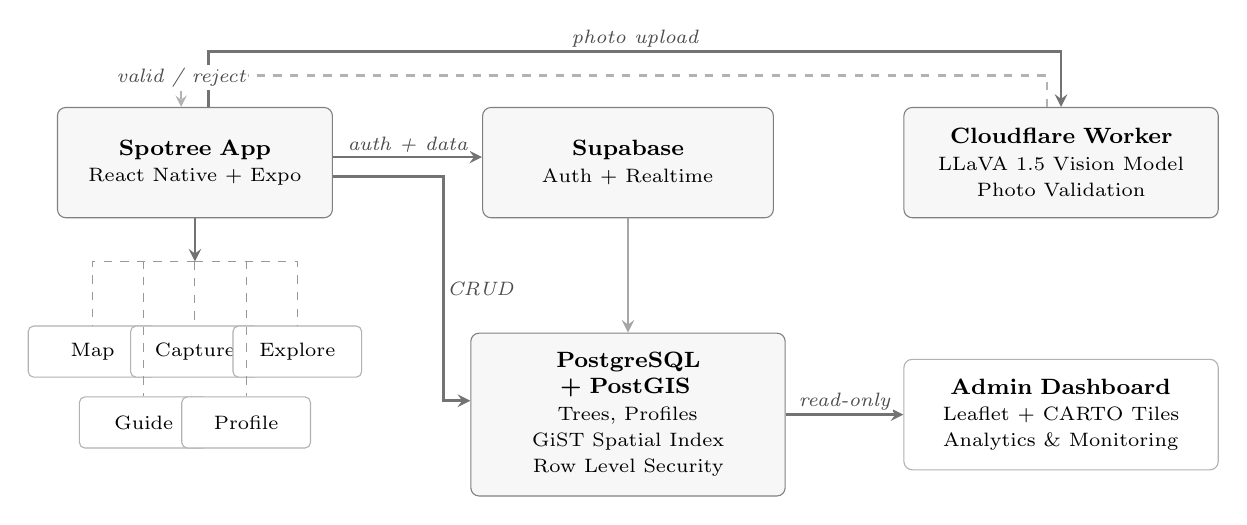
\begin{tikzpicture}[
  box/.style={draw=black!50, fill=spotbg, rounded corners=3pt, minimum height=1.4cm, align=center, font=\footnotesize, inner sep=7pt},
  screenbox/.style={draw=black!30, fill=white, rounded corners=2pt, minimum height=0.65cm, text width=1.4cm, align=center, font=\scriptsize},
  arr/.style={->, line width=1pt, black!55, >=stealth},
  darr/.style={->, line width=0.8pt, black!30, >=stealth, dashed},
  lbl/.style={font=\scriptsize\itshape, black!70, fill=white, inner sep=1pt},
]

% ── Top row ──
\node[box, text width=3cm] (app) at (0, 0)
  {\textbf{Spotree App}\\{\scriptsize React Native + Expo}};

\node[box, text width=3.2cm] (supa) at (5.5, 0)
  {\textbf{Supabase}\\{\scriptsize Auth + Realtime}};

\node[box, text width=3.5cm] (ai) at (11, 0)
  {\textbf{Cloudflare Worker}\\{\scriptsize LLaVA 1.5 Vision Model}\\{\scriptsize Photo Validation}};

% ── Bottom row ──
\node[box, text width=3.5cm, minimum height=1.7cm] (db) at (5.5, -3.2)
  {\textbf{PostgreSQL + PostGIS}\\{\scriptsize Trees, Profiles}\\{\scriptsize GiST Spatial Index}\\{\scriptsize Row Level Security}};

\node[box, text width=3.5cm, fill=white, draw=black!30] (admin) at (11, -3.2)
  {\textbf{Admin Dashboard}\\{\scriptsize Leaflet + CARTO Tiles}\\{\scriptsize Analytics \& Monitoring}};

% ── Screen sub-boxes ──
\node[screenbox] (s1) at (-1.3, -2.4) {\scriptsize Map};
\node[screenbox] (s2) at (0, -2.4) {\scriptsize Capture};
\node[screenbox] (s3) at (1.3, -2.4) {\scriptsize Explore};
\node[screenbox] (s4) at (-0.65, -3.3) {\scriptsize Guide};
\node[screenbox] (s5) at (0.65, -3.3) {\scriptsize Profile};

% Single arrow from app, then dashed lines branching to each screen
\draw[arr] (app.south) -- ++(0,-0.55) coordinate (branch);
\draw[black!40, dashed] (branch) -| (s1.north);
\draw[black!40, dashed] (branch) -- (s2.north);
\draw[black!40, dashed] (branch) -| (s3.north);
\draw[black!40, dashed] (branch) -| (s4.north);
\draw[black!40, dashed] (branch) -| (s5.north);

% ── Arrows ──

% App → Supabase
\draw[arr] ([yshift=2pt]app.east) -- node[lbl, above] {auth + data} ([yshift=2pt]supa.west);

% App → DB (goes right then down)
\draw[arr] ([yshift=-5pt]app.east) -- ++(1.4,0) |- node[lbl, right, pos=0.25] {CRUD} ([yshift=5pt]db.west);

% Supabase → DB
\draw[arr, black!35] (supa.south) -- (db.north);

% App → AI (photo upload over the top)
\draw[arr] ([xshift=5pt]app.north) -- ++(0,0.7) -| node[lbl, above, pos=0.25] {photo upload} (ai.north);

% AI → App (dashed response back)
\draw[darr] ([xshift=-5pt]ai.north) -- ++(0,0.4) -| node[lbl, above, pos=0.75] {valid / reject} ([xshift=-5pt]app.north);

% DB → Admin
\draw[arr] (db.east) -- node[lbl, above] {read-only} (admin.west);

\end{tikzpicture}
\end{center}
\vspace{0.3cm}

\subsection{Tech Stack}

\begin{center}
\proposalTableStart
\begin{tabularx}{\textwidth}{|>{\raggedright\arraybackslash}p{0.27\textwidth}|Y|}
\hline
\proposalTableHeader
\textbf{Component} & \textbf{Technology} \\
\hline
Mobile App & React Native + Expo SDK 54, TypeScript \\
\hline
Authentication & Supabase Auth (email/password) \\
\hline
Database & PostgreSQL + PostGIS (via Supabase) \\
\hline
Spatial Data & \texttt{geography(Point, 4326)} with GiST spatial index \\
\hline
AI Validation & Cloudflare Workers AI --- LLaVA 1.5 vision-language model \\
\hline
AI Proxy & Cloudflare Worker (keeps API keys server-side) \\
\hline
Image Processing & expo-image-manipulator (resize/compress before AI) \\
\hline
Maps (App) & react-native-maps (Apple Maps / Google Maps) \\
\hline
Maps (Admin) & Leaflet.js + CARTO dark tile layer \\
\hline
Admin Dashboard & Single-file HTML/JS --- zero build step \\
\hline
\end{tabularx}
\proposalTableEnd
\end{center}

% ══════════════════════════════════════════════════════════════
\clearpage
\section{OGC Compliance \& Data Export}

All tree data is stored in a \textbf{PostGIS} database using the standard \texttt{geography(Point, 4326)} type --- WGS84 coordinate reference system, the global standard for GPS data and OGC-compliant spatial systems.

This means the data can be exported directly in standard GIS formats:

\begin{center}
\proposalTableStart
\begin{tabularx}{\textwidth}{|>{\raggedright\arraybackslash}p{0.22\textwidth}|>{\raggedright\arraybackslash}p{0.28\textwidth}|Y|}
\hline
\proposalTableHeader
\textbf{Format} & \textbf{Method} & \textbf{Use Case} \\
\hline
GeoJSON & \texttt{ST\_AsGeoJSON()} or API & Web mapping, API integration, lightweight exchange \\
\hline
Shapefile & \texttt{pgsql2shp} or QGIS & Traditional GIS software (ArcGIS, QGIS), municipal systems \\
\hline
GeoParquet & \texttt{ogr2ogr} with Parquet driver & Modern columnar format for large-scale spatial analytics \\
\hline
WFS/WMS & GeoServer or pg\_featureserv & OGC web services for SDI infrastructure integration \\
\hline
\end{tabularx}
\proposalTableEnd
\end{center}

The database schema uses a \textbf{spatial index} (GiST) on the tree locations for efficient spatial queries --- bounding box lookups, nearest-neighbor searches, and spatial joins with existing Munich geodata layers.

\textbf{Integration path:} Munich's GeodataService can connect directly to the PostGIS database via standard drivers, or consume exported files in their preferred format. The \texttt{trees\_with\_user} view provides a clean, denormalized dataset ready for analysis.

% ══════════════════════════════════════════════════════════════
\clearpage
\section{Co-Creation Phase Roadmap}

The current prototype demonstrates the core concept and technical feasibility. The co-creation phase will expand Spotree into a production-ready platform.

\subsection{Gamification \& Reward System}

\textbf{Leaderboard:} A public ranking of top contributors by trees spotted, species identified, and data quality (based on confidence scores and verification by other students). Visible in-app to drive friendly competition.

\textbf{Area Ownership:} Students can ``own'' a neighborhood zone (by postal code) by being the top contributor in that area. If another student maps more trees or provides higher-quality data in the same zone, ownership transfers. This creates ongoing engagement --- students return to defend their territory and fill in gaps. It directly addresses the challenge goal of strengthening neighbourhood connection: students develop a sense of responsibility for ``their'' zone's tree data.

\textbf{Badges \& Milestones:} Unlock achievements for first tree, first species ID, mapping in multiple neighborhoods, seasonal mapping (capturing the same tree across seasons), etc.

\subsection{AI-Powered Species Classification}
\label{sec:ai-species}

The current prototype uses AI to validate that photos contain trees. The co-creation phase will add \textbf{automatic species identification}:

\subsubsection{Approach}
\begin{enumerate}
  \item \textbf{Ground truth collection} --- Use the prototype to collect GPS-tagged, species-labeled photos from students. Each photo has a species label and confidence score, giving us a quality-weighted training dataset.
  \item \textbf{Seasonal variation} --- Munich trees look significantly different across seasons (leaf-on vs.\ leaf-off, flowering periods, autumn colors). We will systematically collect images across all four seasons. A model trained only on summer photos would fail in winter.
  \item \textbf{Munich-specific training} --- Urban trees in Munich may look different from the same species in a forest or another climate zone. Local training data ensures the model reflects actual conditions.
  \item \textbf{Model options:}
  \begin{itemize}
    \item Fine-tune an open-source vision model on Munich-specific data
    \item Evaluate existing providers (Pl@ntNet API, iNaturalist model) for baseline accuracy
    \item Focus custom training on species where existing models struggle
  \end{itemize}
  \item \textbf{In-app flow:} After the student takes a photo, the AI suggests a species with a confidence score. The student can accept, correct, or mark as ``Not Sure.'' Corrections feed back into the training loop.
\end{enumerate}

\subsubsection{Continuous Learning from Student Data}

Every tree submitted through Spotree becomes a potential training sample. The species label paired with the student's confidence score acts as a \textbf{soft label} --- a submission with 95\% confidence is a stronger training signal than one at 40\%. As the database grows, we can:

\begin{itemize}
  \item Filter high-confidence submissions (e.g., $>$80\%) as reliable ground truth for model retraining
  \item Use cross-verified entries (same tree, same species from multiple students) as gold-standard labels
  \item Retrain or fine-tune the model periodically with the latest data, so it improves as more students contribute
  \item Track model accuracy over time by comparing AI predictions against student consensus
\end{itemize}

This creates a \textbf{virtuous cycle}: students collect data, data trains the model, the model helps future students identify species more accurately, and those students submit even better-labeled data. The more Spotree is used, the smarter it gets.

\subsection{Location Accuracy \& Camera-to-Tree Distance}

A photo's GPS tag records \textit{where the camera was}, not where the tree is. If a student photographs a tree from 20 meters away, the mapped coordinate could be significantly offset from the actual trunk location. For GeodataService Munich, positional accuracy is critical --- duplicate detection, cross-referencing with existing tree cadastres, and spatial joins all depend on coordinates being close to the true tree position.

The co-creation phase will investigate and implement a methodology for ensuring location accuracy:

\subsubsection{Distance Estimation}
\begin{itemize}
  \item \textbf{Monocular depth estimation} --- Use a lightweight depth model (e.g., MiDaS or Depth Anything) to estimate the camera-to-tree distance from a single photo. The tree trunk can be identified as the primary foreground object, and its relative depth converted to an approximate metric distance using known camera parameters (focal length from EXIF).
  \item \textbf{Object size heuristics} --- If the student has already estimated trunk diameter or tree height, these physical dimensions combined with their pixel size in the image provide a second distance estimate via basic photogrammetry.
  \item \textbf{Threshold enforcement} --- Define a maximum acceptable camera-to-tree distance (e.g., 5--10 meters). If the estimated distance exceeds this threshold, prompt the student: \textit{``You seem far from the tree --- please move closer for a more accurate location.''} This nudge improves data quality at the point of capture.
\end{itemize}

\subsubsection{Coordinate Correction}
\begin{itemize}
  \item \textbf{Bearing-based offset} --- Using the device compass heading at capture time and the estimated distance, compute a corrected coordinate that shifts the GPS point from the camera position toward the tree along the viewing direction.
  \item \textbf{Multi-observation averaging} --- When multiple students photograph the same tree from different positions, triangulating their corrected coordinates produces a more accurate consensus location.
  \item \textbf{Accuracy metadata} --- Store the estimated camera-to-tree distance and correction method as metadata alongside each tree entry, giving GeodataService a per-record quality indicator for positional accuracy.
\end{itemize}

This investigation is directly relevant to the team's expertise: Jayendra's work on geospatial data pipelines and Hari's research on image-based geolocation (ICLR 2026) provide the methodological foundation for building robust distance estimation and coordinate correction into Spotree.

\subsection{Educational Earth Observation Module}

A new tab in the Spotree Guide showing \textbf{how tree species appear from different sensors and perspectives:}

\begin{itemize}
  \item \textbf{High-resolution satellite imagery} --- What does a cluster of this species look like from orbit? (Using freely available Sentinel-2 or commercial VHR imagery)
  \item \textbf{Hyperspectral views} --- How does the spectral signature of this species differ from others? This introduces students to the concept that sensors can ``see'' beyond visible light
  \item \textbf{LiDAR point clouds} --- 3D structure of tree canopies, connecting to the height and diameter measurements students make on the ground
  \item \textbf{Seasonal comparisons} --- Same location across seasons from satellite, showing phenological changes
\end{itemize}

This bridges the gap between ground-level observation and remote sensing, introducing students to how cities actually monitor urban forests at scale. Space and satellite technology is inherently exciting for students and adds a unique educational dimension beyond traditional biology lessons.

\subsection{Platform Scalability}

The Spotree architecture is \textbf{not limited to trees}. The same capture-validate-map-explore pattern can be extended to other urban assets:

\begin{itemize}
  \item \textbf{Public benches} --- location, condition, accessibility
  \item \textbf{Table tennis tables} --- public sports infrastructure mapping
  \item \textbf{Playgrounds} --- equipment inventory and condition
\end{itemize}

Each asset type gets its own capture form, guide section, and map layer. The database schema, admin dashboard, and gamification system remain the same. This makes Spotree a general-purpose \textbf{crowdsourced urban data collection platform} that starts with trees and grows with the city's needs.

\subsection{Production Infrastructure}

The current prototype runs on Supabase's free tier. For production deployment:

\begin{center}
\proposalTableStart
\begin{tabularx}{\textwidth}{|>{\raggedright\arraybackslash}p{0.25\textwidth}|>{\raggedright\arraybackslash}p{0.25\textwidth}|Y|}
\hline
\proposalTableHeader
\textbf{Component} & \textbf{Technology} & \textbf{Hosting} \\
\hline
Mobile App & React Native (iOS + Android) & App Store / Play Store \\
\hline
App Backend API & Dedicated service & Hetzner Cloud (German-based) \\
\hline
Database & PostgreSQL + PostGIS & Hetzner Cloud \\
\hline
DB Admin & pgAdmin & Hetzner Cloud \\
\hline
Analytics & Grafana (connected to PostGIS) & Hetzner Cloud \\
\hline
AI Service & Dedicated inference service & Hetzner Cloud / Cloudflare \\
\hline
\end{tabularx}
\proposalTableEnd
\end{center}

\textbf{Why Hetzner:} German-based hosting ensures GDPR compliance with data residency in Germany. No dependency on external SaaS providers --- full control over the data pipeline. Microservice architecture allows independent scaling of each component.

\textbf{Why self-hosted Grafana:} Professional-grade monitoring with alerting, time-series analysis, custom queries, and multi-user access control. City staff can build their own dashboards without developer involvement.

During the co-creation phase, we will actively visit Munich schools to present and demonstrate Spotree, ensuring students and teachers across the city know about the app and how to use it for real data collection.

\vspace{1cm}
\begin{center}
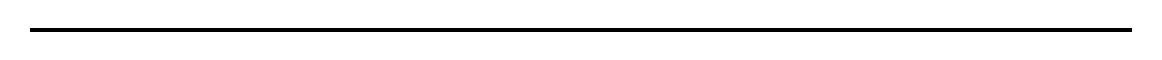
\begin{tikzpicture}
\draw[spotlight, line width=1.5pt] (0,0) -- (14,0);
\end{tikzpicture}
\end{center}

\end{document}
